In this lab, the Fourier Transform was explored by means of the use of the FFT button on the oscilloscope. The Fourier Transform is a mathematical tool that allows us to convert a signal from the time domain to the frequency domain, thereby allowing the extraction of the frequency components that make up a signal.

A continuous time signal can be described by a sum of sinusoids of different frequencies, amplitudes, and phases. The Fourier Series is a mathematical tool that allows us to decompose a periodic signal into a sum of sinusoids, to use it, however, it must first be established what it means for a signal to be periodic.
We say that a signal is periodic if for some positive period $T$ the following holds:
\begin{equation}
    x(t) = x(t + nT)
\end{equation}
This must hold for all $t$. The fundamental period is the smallest positive period $T$ for which the above holds. The fundamental frequency is defined as:

\begin{equation}
    \omega_0 = \frac{2\pi}{T}
\end{equation}

To determine the complex Fourier Series coefficients, the following equation is used,
\begin{equation}
    c_\nu = \frac{1}{T}\int_{T}f(t)e^{-j\nu\omega_0t}dt
\end{equation}
Where $f(t)$ can then be expressed as,
\begin{equation}
    f(t) = \sum_{\nu=-\infty}^{+\infty}c_\nu e^{j\nu\omega_0t}
\end{equation}
Where the DC component is obtained by substituting $\nu = 0$.
\begin{equation}
    c_0 = \frac{1}{T}\int_{T}f(t)dt
\end{equation}
\newpage
The signal does not have to be represented by complex exponentials, indeed, it can also be represented by sines and cosines, where the fourier coefficients $a_0$, $a_\nu$, and $b_\nu$ are used.
\begin{equation}
    f(t) = \frac{a_0}{2} + \sum_{\nu=1}^{+\infty}a_\nu \cos(\nu\omega_0t) + b_\nu\sin(\nu\omega_0t)
\end{equation}

\section{The Square Wave}
\begin{figure}[H]
    \centering
    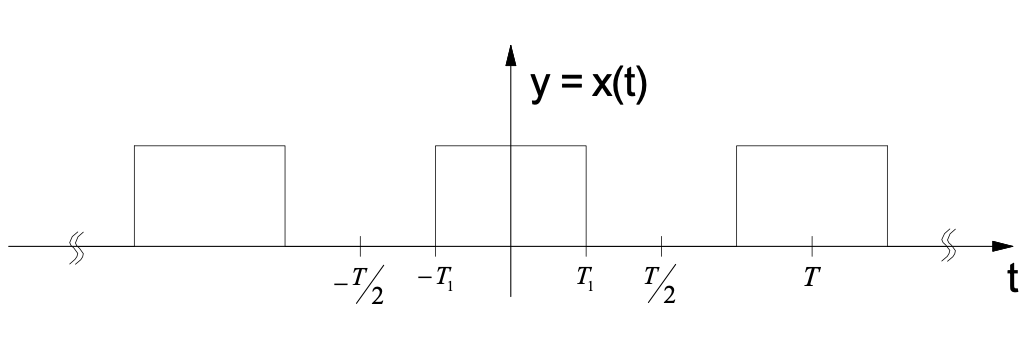
\includegraphics[width=0.8\linewidth]{images/square_wave.png}
    \caption{Square Wave}
    \label{fig:square_wave}
\end{figure}
The square wave shown is a periodic signal that is defined as follows:
\begin{equation}
    x(t) = \begin{cases}
        1 & \text{if } |t| \leq T/2    \\
        0 & \text{if } T_1 < |t| < T/2
    \end{cases}
\end{equation}
Using the equations for the Fourier Series coefficients, and knowing the signal is $1$ between $-T/4$ and $T/4$, and $0$ elsewhere,
\begin{equation}
    c_0 = \frac{1}{T}\int_{-T/2}^{T/2}x(t) dt = \frac{1}{T}\int_{-T/4}^{T/4} 1 dt = \frac{1}{T}\left(\frac{T}{4} - \left(-\frac{T}{4}\right)\right) = \frac{1}{2} \\
\end{equation}
For the $c_\nu$ coefficients,
\begin{equation}
    \begin{gathered}
        c_\nu = \frac{1}{T}\int_{-T_1}^{T_1}x(t)e^{-j \nu\omega_0t} dt \\
        = -\frac{1}{j\nu\omega_0T}e^{-j\nu\omega_0t}\Big|_{-T_1}^{T_1} \\
        = \frac{2}{\nu\omega_0T}\left(\frac{e^{j\nu\omega_0T_1} - e^{-j\nu\omega_0T_1}}{2j}\right)
    \end{gathered}
\end{equation}
Where from Euler's identities, it can be extracted:
\begin{equation}
    c_\nu = \frac{1}{\nu\pi}\sin(\nu\omega_0T_1)
\end{equation}
Where $T$ is the period, and $T_1$ is the width of the pulses.
Similarly, for the $a_\nu$ and $b_\nu$ coefficients extracted from the complex exponential form of the Fourier Series,
\begin{equation}
    a_\nu = 2\Re(c_\nu) = \frac{2}{\nu\pi}\sin\left(\nu\frac{\pi}{2}\right) = \begin{cases}
        0                & {\nu \text{ even}} \\
        \frac{2}{\nu\pi} & {\nu \text{ odd}}
    \end{cases}
\end{equation}
\begin{equation}
    b_\nu = -2\Im(c_\nu) = 0
\end{equation}

Which leads to,
\begin{equation}
    x(t) = \frac{1}{2} + \frac{2}{\pi}\sum_{\nu=1,3,5,...}^{\infty}sin(\nu\frac{\pi}{2})\cdot\frac{cos(\nu\omega_0t)}{\nu}
\end{equation}

The Gibbs Phenomenon is the overshoot of the Fourier Series approximation near the discontinuities of a periodic signal, which most surely can be observed in the case of the square wave. The discontinuities in the pulses makes it necessary to have more and more sinusoids to approximate it, and even then, the approximation is not perfect, leading to "ringing" near the discontinuities.

\begin{figure}[H]
    \centering
    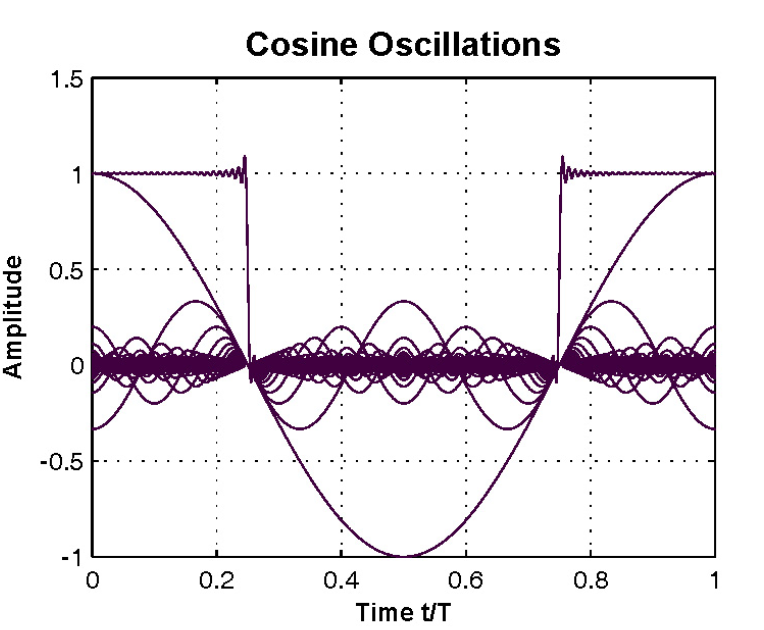
\includegraphics[width=0.8\linewidth]{images/gibbs_phenomenon.png}
    \caption{\centering Gibbs Phenomenon, the overshoot near the discontinuities of the square wave approximated by 50 sinusoids.}
    \label{fig:gibbs_phenomenon}
\end{figure}

\section{The Fourier Transform}

The Continuous Time Fourier Transform is what is obtained when the period of the Fourier Series goes to infinity.
It is defined by,
\begin{equation}
    X(j\omega) = \int_{\infty}^{\infty}x(t)e^{-j\omega t}dt
\end{equation}
And the inverse is given by,
\begin{equation}
    x(t) = \frac{1}{2\pi}\int_{\infty}^{\infty}x(t)e^{j \omega t}d\omega
\end{equation}
For a square pulse, which is essentially a square wave of infinite period, the Fourier Transform is given by,
\begin{equation}
    X(j\omega) = \int_{-\tau/2}^{\tau/2}e^{-j\omega t} dt
\end{equation}

By using Euler's trigonometric identities, it is obtained that the Fourier Transform of the square pulse is given by,
\begin{equation}
    X(j\omega) = \tau \cdot \left[\frac{\sin(\frac{\omega \tau}{2})}{\frac{\omega \tau}{2}}\right] = \tau \cdot sinc\left(\frac{\omega \tau}{2}\right)
\end{equation}
\section{The Discrete Fourier Series}
The Discrete Fourier Series is the discrete time equivalent of the Fourier Series, and the coefficients are defined as follows:
\begin{equation}
    a_\nu = \frac{1}{N}\sum_{n=-N_1}^{N_1}e^{-j\frac{2\pi\nu n}{N}}
\end{equation}
Furthermore, the fourier series summation can be expressed as,
\begin{equation}
    x[n] = \frac{1}{N}\sum_{\nu=(N)}a_\nu e^{j\frac{2\pi\nu n}{N}}
\end{equation}
\section{The Discrete Fourier Transform}
Because computers can not handle continuous time signals, an analogous transform to the Fourier Transform is necessary, one that can handle discrete time signals. This is the Discrete Fourier Transform, which is defined as follows:
\begin{equation}
    X[k] = \sum_{n=0}^{N-1}x[n]e^{-j\frac{2\pi kn}{N}}
\end{equation}
And the inverse is given by,
\begin{equation}
    x[k] = \frac{1}{N}\sum_{n=0}^{N-1}X[n]e^{j\frac{2 \pi kn}{N}}
\end{equation}
The DFT, and the more commonly used algorithm to perform the DFT, the FFT, are widely used for signal filtering, for correlation analysis and for spectral analysis. The FFT simply uses the properties of periodicity, symmetry, and uses a divide-and-conquer approach to reduce the number of computations needed to perform the DFT. It is not an approximation of the DFT, it is simply a more efficient way to compute it.

During the experiment, the Hanning Window is used on the oscilloscope as it is the best window to use when the signal is periodic. A window function simply cuts out the signal so that the FFT can be performed on it. The Hanning Window is some sort of rectangular pulse multiplied by the time signal, however, which leads to a sinc in the frequency domain. It will affect the transform, but it is the only viable option to perform the FFT on the signal.